The Acoustic\-A\-V\-E library (libaave) is an auralisation library. It is the equivalent of a 3\-D graphics visualisation library, but for audio\-: given a model of a room, the positions of the sound sources, the position and head orientation of the listener, and the anechoic audio stream of each sound source, libaave produces the 3\-D binaural soundfield that would be heard by that listener in that virtual environment.


\begin{DoxyImage}
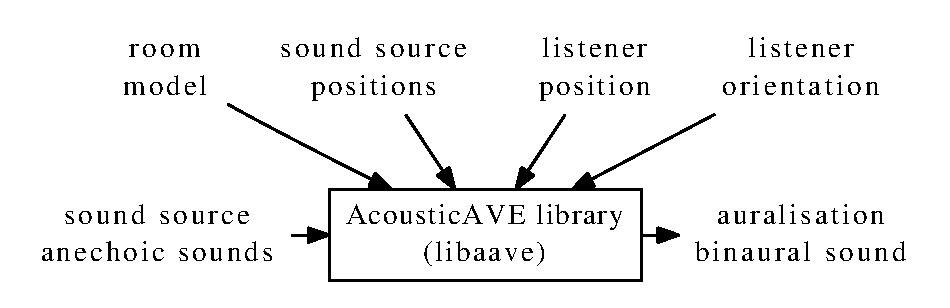
\includegraphics{libaave}
\caption{Role of the Acoustic\-A\-V\-E library}
\end{DoxyImage}
 libaave supports moving sound sources and listener, therefore it can be used for auralisation of interactive virtual reality environments, usually in combination with a 3\-D graphics visualisation library.

libaave performs in real-\/time for virtual rooms of some complexity (number of surfaces) and some order of sound reflections (configured by the user), more specifically the total number of sounds, that depend on the processor used. Benchmarks\-:
\begin{DoxyItemize}
\item Intel Atom N2600 1.\-6\-G\-Hz\-: 66 sounds
\item Intel Xeon 2\-G\-Hz\-: 89 sounds
\item A\-M\-D Opteron 248 2.\-2\-G\-Hz\-: 193 sounds
\end{DoxyItemize}

The following diagrams illustrate typical usages of the Acoustic\-A\-V\-E library for developing auralisation programs, one single-\/threaded and one multi-\/threaded.


\begin{DoxyImage}
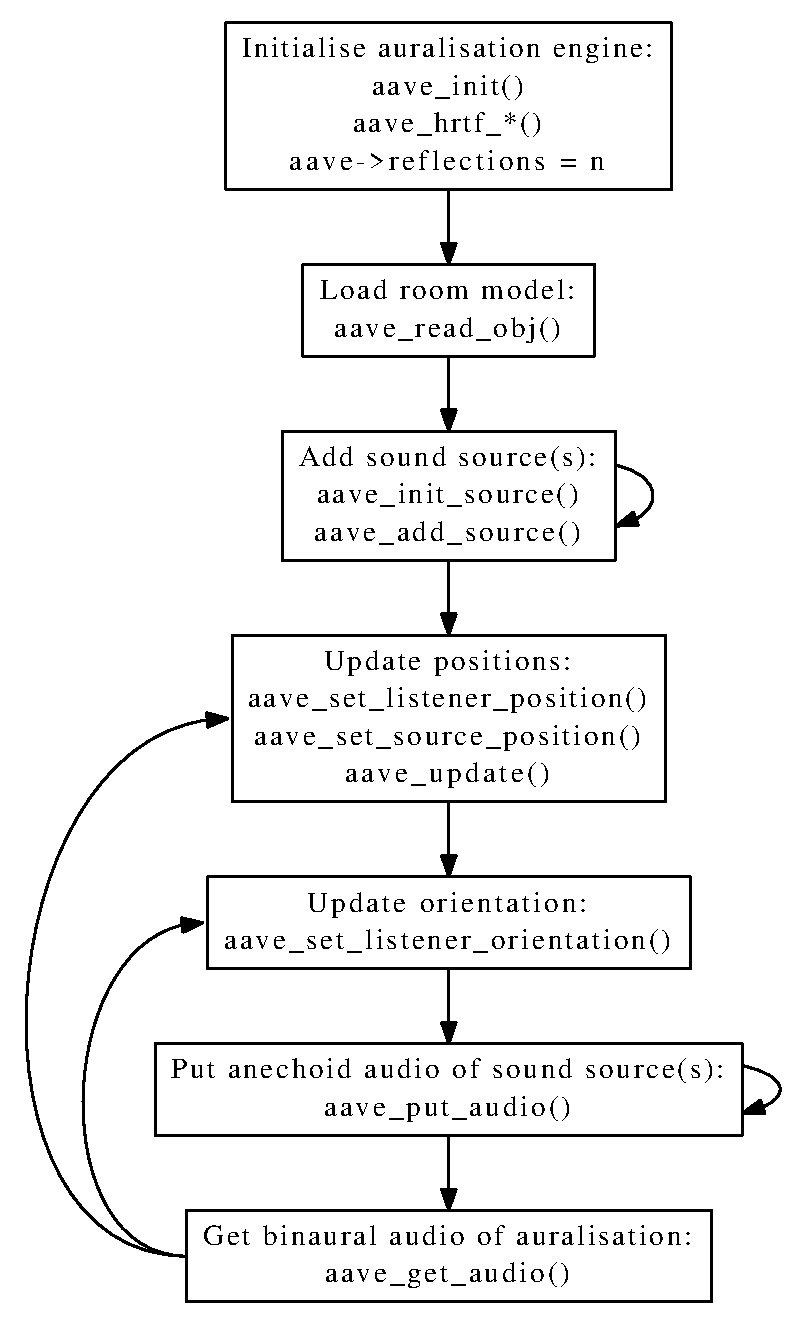
\includegraphics{usage1}
\caption{Single-\/thread usage example}
\end{DoxyImage}
 
\begin{DoxyImage}
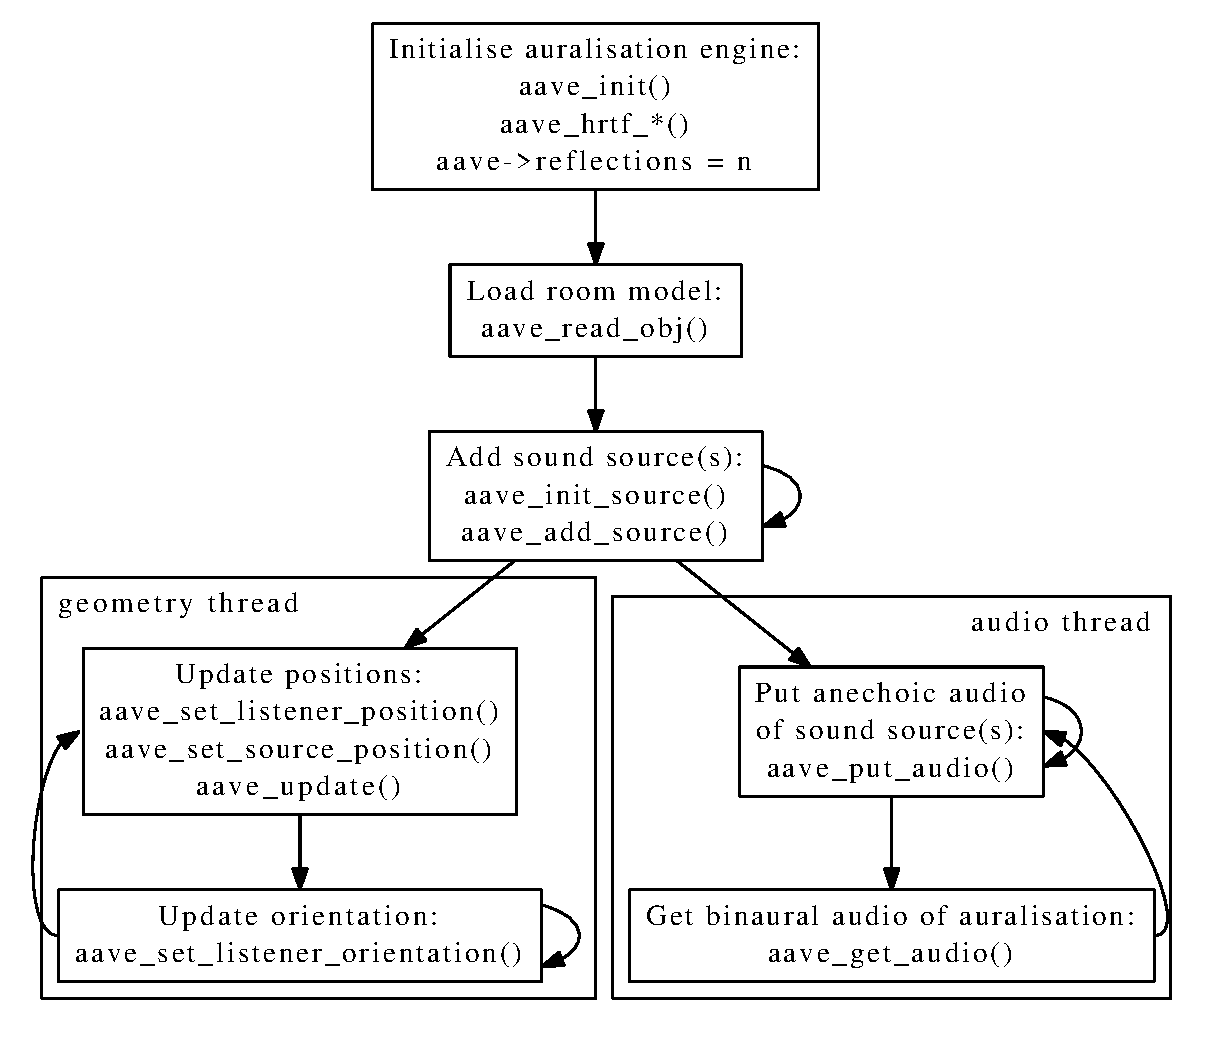
\includegraphics[width=\textwidth]{usage2}
\caption{Multi-\/thread usage example}
\end{DoxyImage}
\hypertarget{index_installation}{}\section{Installation}\label{index_installation}
libaave is implemented in A\-N\-S\-I C and does not depend on any external library, so it is fairly portable (it is known to work on G\-N\-U/\-Linux and Microsoft Windows systems, but should also work on any other platform with an A\-N\-S\-I C compiler).
\begin{DoxyEnumerate}
\item Download the source code\-: 
\begin{DoxyCode}
git clone https:\textcolor{comment}{//code.ua.pt/git/acousticave}
\end{DoxyCode}

\item Build libaave\-: 
\begin{DoxyCode}
cd acousticave/libaave
make
\end{DoxyCode}

\end{DoxyEnumerate}

For a quick start on using libaave in your programs, see the examples in acousticave/libaave/examples/.\hypertarget{index_coordinates}{}\section{Coordinates}\label{index_coordinates}
For all 3\-D points (positions and room model vertices), libaave uses the coordinate system commonly used by C\-A\-D architecture programs\-: x=North, y=West, z=up, in metres.

For the listener head orientation angles, libaave uses the coordinate system commonly used by inertial sensors\-: x=North, y=East, z=down, in radians. This means\-:
\begin{DoxyItemize}
\item roll $>$ 0 is tilt right, roll $<$ 0 is tilt left
\item pitch $>$ 0 is tilt up, pitch $<$ 0 is tilt down
\item yaw $>$ 0 is rotate right, yaw $<$ 0 is rotate left, yaw = 0 is North
\end{DoxyItemize}\hypertarget{index_overview}{}\section{Overview}\label{index_overview}
The file \hyperlink{aave_8h}{aave.\-h} is the public header file of libaave. Include it from your program source files to use its structures and functions.

The file \hyperlink{geometry_8c}{geometry.\-c} implements all functions related to geometry processing\-: construction of the 3\-D room model, coordinate conversions, determining the image-\/source positions, the sound reflection paths, the audible and non-\/audible sound paths, and passing all this information to the audio processing functions.

The file \hyperlink{obj_8c}{obj.\-c} contains a convenience function that reads a 3\-D model from a Wavefront .O\-B\-J file and calls the appropriate functions in \hyperlink{geometry_8c}{geometry.\-c} to construct the room to be auralised in just one step.

The file \hyperlink{audio_8c}{audio.\-c} implements the core of the audio processing\-: receiving anechoic audio data from the sound sources, head-\/related transfer function (H\-R\-T\-F) processing, and generating the corresponding auralised audio data in binaural format.

The files \hyperlink{hrtf__cipic_8c}{hrtf\-\_\-cipic.\-c}, \hyperlink{hrtf__listen_8c}{hrtf\-\_\-listen.\-c}, \hyperlink{hrtf__mit_8c}{hrtf\-\_\-mit.\-c}, and \hyperlink{hrtf__tub_8c}{hrtf\-\_\-tub.\-c} implement the interface functions for using the C\-I\-P\-I\-C, L\-I\-S\-T\-E\-N, M\-I\-T, and T\-U-\/\-Berlin H\-R\-T\-F sets, respectively.

The files \hyperlink{dft_8h}{dft.\-h} and \hyperlink{idft_8h}{idft.\-h} implement the Discrete Fourier Transform and Inverse Discrete Fourier Transform algorithms, respectively, used mainly for the H\-R\-T\-F processing.

The file \hyperlink{material_8c}{material.\-c} implements the functions related to the sound absorption caused by the different surface materials\-: the table of material reflection coefficients by frequency band, the table lookup, and the design of the audio filters.

The file reverb.\-c implements a simple artificial reverberation algorithm that adds a tail of late reflections to the auralisation output. The file \hyperlink{reverb__dattorro_8c}{reverb\-\_\-dattorro.\-c} implements the Dattorro reverberator.

The directory tools contains the programs used to automatically generate the hrtf\-\_\-$\ast$\-\_\-set$\ast$.c source files from the respective H\-R\-T\-F data sets, the dftsincos.\-c source file with the sin() and cos() lookup table for the D\-F\-T and I\-D\-F\-T algorithms, and miscellaneous utility programs to handle or generate audio files.

The directory tests/ contains programs to verify the correctness of the functions implemented in libaave.

The directory examples/ contains programs to show how libaave can be used for different auralisation applications.

The directory doc/ contains the files to generate this document from the documentation written in the source files.\hypertarget{index_acknowledgements}{}\section{Acknowledgements}\label{index_acknowledgements}
The development of libaave was funded by the Portuguese Government through F\-C\-T (Fundação para a Ciência e a Tecnologia) as part of the project Acoustic\-A\-V\-E\-: Auralisation Models and Applications for Virtual Reality Environments (P\-T\-D\-C/\-E\-E\-A-\/\-E\-L\-C/112137/2009). 